\documentclass[11pt,a4paper]{article}
% WHALEFALL -- Zenodo preprint, version 3 (draft, 26 October 2026).  Build: latexmk -pdf main-v3.tex
% Versions 1 (main.tex, 11 October 2026) and 2 (main-v2.tex, 25 October 2026) are kept unchanged for comparison;
% what changed is listed in Secs. "What changed since version 2" and "What changed since version 1".
\usepackage[margin=2.4cm]{geometry}
% T1 fontenc omitted: cm-super not available in the build environment
\usepackage[utf8]{inputenc}
\usepackage{amsmath,amssymb}
\usepackage{graphicx}
\usepackage{booktabs}
\usepackage{array}
\usepackage{longtable}
\newcolumntype{L}[1]{>{\raggedright\arraybackslash}p{#1}}
\usepackage{xcolor}
\usepackage[numbers,sort&compress]{natbib}
\usepackage[colorlinks=true,linkcolor=blue!50!black,citecolor=blue!50!black,urlcolor=blue!50!black]{hyperref}
\usepackage[expansion=false]{microtype}
\usepackage{caption}
\usepackage{orcidlink}
\usepackage{url}
\captionsetup{font=small,labelfont=bf}

\newcommand{\RP}{\mathbb{RP}^3}
\newcommand{\Ztwo}{\mathbb{Z}_2}
\newcommand{\Mpl}{M_{\rm Pl}}
\newcommand{\RG}{R_\Gamma}
\newcommand{\Rxi}{R_\xi}
\newcommand{\dA}{\delta A}
\newcommand{\Xu}{X_{\rm univ}}
\newcommand{\todo}[1]{\textcolor{red}{[#1]}}

\title{\textbf{WHALEFALL: a preregistered, falsifiable toy cosmology from a quasi-topological bounce to cold dark matter from the collapse of an $\RP$ string--wall network}}
\author{Jose Bautista\,\orcidlink{0009-0001-6655-4028}\thanks{\href{mailto:jozebautista@gmail.com}{jozebautista@gmail.com}}}
\date{October 26, 2026}

\begin{document}
\maketitle

\begin{abstract}
WHALEFALL is a toy cosmology built as a single chain of computations, from a non-singular beginning to a dark-matter prediction, with every verdict-bearing computation preregistered and reproducible.
A small, closed, contracting patch bounces through a non-polynomial quasi-topological gravity core, which kicks a scalar onto an inflationary plateau, where it either enters stochastic eternal inflation or inflates directly; either way the observable universe has $n_s=0.9728$ and $r=0.0050$.
A symmetric-tensor order parameter orders into an $\RP$ vacuum and leaves a network of global $\Ztwo$ strings; a small explicit breaking gives the Goldstones a mass $m_G$, and the network collapses as string--wall systems when $H\simeq m_G/3$.
This second version replaces the dark sector of version~1.
(i) The plateau is now a standard order-four pole, with the same cosmic microwave background (CMB) predictions and the same statistics of eternal births as the postulated ten-level hierarchy of version~1.
(ii) The lattice comparison of the $\RP$ and U(1) networks is consolidated: density ratio $\Rxi\simeq1.6$, emission ratio $\RG=1.56\pm0.12$ with the initial massive bath drained, and an emission slope compatible with $1$.
(iii) The dark matter is set not by the string radiation but by the collapse, which holds $10^2$--$10^3$ times the misalignment energy. We measure it on the lattice: at one lattice size $\RP$ and U(1) leave the same soft population per unit string energy, and its string-independent soft momentum grows with $\ell=\ln(m_r/H)$ as $\ell^{1.35\pm0.31}$ across four lattice sizes with twelve networks each, which extrapolates to $\Xu\simeq560$ ($244$--$1370$) at the cosmological $\ell\simeq90$.
(iv) The decay constant $F$ is a free parameter below a ceiling $F_0=1.07\times10^{15}$\,GeV, the value fixed in version~1. Passing the measured population through a patched CLASS with Lyman-$\alpha$ gates, together with observational isocurvature bounds, black-hole superradiance, dark radiation and CMB string bounds, leaves a band whose upper edge falls with $\Xu$: $0.5F_0$ at the central extrapolation and $0.35$--$0.85F_0$ over the whole interval, with a lower edge at $0.03$--$0.09F_0$.
(v) A full Lyman-$\alpha$ likelihood with the cosmology and the intergalactic medium marginalised excludes $F_0$ even in the most favourable case tested and confirms the $0.7F_0$ edge at $\Xu\simeq320$.
This third version adds the coherence of the parent's bounces under perturbations of inflationary amplitude. Evolving the parent through its bounce with dust and an inhomogeneous inflaton gives, in a preregistered test, the same tolerance as a dust model: $12$--$18\%$ of fertile births are direct, non-eternal children that bounce coherently and need the plateau flat only up to their landing value, against $1.8$--$2.9\%$ for eternal children.
The best estimate is cold pseudo-Goldstone dark matter, $96$--$99\%$ of it from the collapse, with $F\approx0.06$--$0.5F_0$, $m_G\approx10^{-17}$--$10^{-13}$\,eV, a small-scale suppression of at most a few per cent at $k=10\,h$/Mpc near the upper edge, white-noise isocurvature below current bounds, $\Delta N_{\rm eff}\lesssim3\times10^{-3}$, and no string signal in LISA.
We list every open assumption, every failed gate and every superseded statement of version~1.
\end{abstract}

\clearpage
\tableofcontents
\bigskip\hrule\bigskip

%=====================================================================
\section{Introduction}
%=====================================================================

Toy cosmologies are usually presented as a sequence of plausible steps, each checked in isolation and often with different parameter choices.
WHALEFALL is an experiment in the opposite direction: a deliberately complete chain, from a non-singular beginning to an observable dark-matter signature, in which
(i) every link is either computed or explicitly declared as an assumption,
(ii) one parameter set is carried through all links (for each value of the free decay constant $F$, \S\ref{sec:F}),
(iii) every computation that yields a verdict is preregistered with its thresholds and verdict logic before it is run, amendments are dated, and failures are reported as such, and
(iv) stages are checked by independent audits that reimplement the essentials rather than reusing the audited code.

The model is the fifth of a series whose four predecessors were discarded by preregistered no-go tests (\S\ref{sec:history}).
It combines ingredients that exist separately in the literature: a non-singular bounce in four-dimensional non-polynomial quasi-topological gravity~\cite{Bueno2025formation,BorissovaMagueijo2026}; an inflationary plateau with an eternal regime; an order parameter with a non-trivial vacuum manifold that produces global strings~\cite{Kibble1976,VilenkinShellard}; and pseudo-Goldstone dark matter from the misalignment of the field and from the network, as in the post-inflationary axion scenario~\cite{GHV2018,GHV2021,Buschmann2022,Hindmarsh2021approach,Saikawa2024,KimParkSon2024,Correia2025spectrum}.

Version~1 of this preprint (11 October 2026) placed the dark matter in the radiation of the string network before its collapse, and made survival hinge on the spectral slope of that radiation at large $\ell$.
Two findings made that picture obsolete.
First, an inventory of the network energy at the time the walls appear shows that the collapse of the string--wall system, which version~1 bracketed as a contribution of order one, carries $10^2$--$10^3$ times the misalignment energy; with it, the emission before the collapse is negligible and the question becomes how much of that energy ends as soft quanta.
Second, the decay constant $F$ that version~1 treated as fixed is a ceiling: the benchmark sits exactly where the dark matter is hottest.
The present version measures the collapse on the lattice, extrapolates it with four lattice sizes, and turns it into a band of $F$ with a chain of preregistered tests that ends in a full Lyman-$\alpha$ likelihood.
Section~\ref{sec:changes} lists every statement of version~1 that no longer holds.
Version~3 adds two preregistered tests of the birth: the coherence of the children that inflate without an eternal phase, and the coherence of the parent's bounces with an inhomogeneous inflaton (\S\ref{sec:birth}); Section~\ref{sec:changes3} lists what they change.

Two results are, as far as we know, new.
The first is methodological: an auditable chain with one parameter set, closed in the sense that every link is either computed or declared as an assumption (it does not demonstrate a recursion of parent and child universes), in which the physical inputs that had to be measured (the emission of the string network and the soft yield of its collapse) were measured, and the input that cannot be measured (their behaviour at $\ell\approx90$) is bracketed and stated as an explicit condition.
The second is a set of lattice measurements for a network of $\Ztwo$ strings with vacuum manifold $\RP\simeq{\rm SO}(3)$ relative to U(1) in the same code: the density and emission ratios, reported in a companion paper~\cite{rp3_paper}, and the soft yield of the string--wall collapse, reported here.

We stress what the paper is not.
It is not a claim that the universe followed this chain.
Several links rest on declared assumptions (\S\ref{sec:open}); the most serious are the flatness of the plateau over a field range of $\sim10^3\Mpl$ if our pocket is eternal, or of $10$--$50\,\Mpl$ if it is a direct child, which conflicts with swampland conjectures in either case, and the explicit symmetry-breaking mass $m_G$, a bare parameter of the effective theory with no ultraviolet origin.
The dark-matter prediction is conditional on extrapolating the collapse from $\ell\lesssim4.4$ to $\ell\approx90$, and we state the interval this leaves.

%=====================================================================
\section{Method: preregistration, audits and a machine-readable contract}
\label{sec:method}
%=====================================================================

Every test that returns a verdict has a specification document written, timestamped and committed before the computation.
It fixes the rows to be computed, the gates and thresholds, and the verdict logic, including what happens if a validation fails, and it writes down the expected outcome.
Later changes are appended as dated amendments; when anything was computed before an amendment, the amendment says so.
Code bugs may be fixed (and are documented); criteria are not changed after seeing the data they decide.
Each verdict is reported even when it goes against the model or against the expectation written beforehand; in this version, for example, the full Lyman-$\alpha$ likelihood excluded the benchmark where its specification expected it to pass (\S\ref{sec:lyafull}), and the expectation of the test that first measured the string--wall collapse was wrong in the other direction; and when the solver preregistered for the coherence test of version~3 turned out unable to cover the contracting patch, it was replaced by a new one, with its own validation gates, through dated amendments before any production run.
Readings made after the data are labelled as informative and never carry a verdict.
Appendix~\ref{app:log} lists every verdict-bearing test of the dark-sector stage with its verdict and its internal code, which indexes the repository~\cite{whalefall_chain}.

Independent re-implementations, written from the specifications in separate sessions without the audited code, audited the first closure tests, the lattice measurements behind the network results, and the Lyman-$\alpha$ likelihood harness; the analyses of the lattice collapse and of the combined band were re-checked in the same way, and both re-checks corrected the wording of a result without changing a verdict.
Four external reviews were answered point by point; several of their claims were rejected after checking them against the code and the data. The audits, and the reviews with their answers, are available from the author on request.
The state of each link is summarised in a machine-readable contract regenerated by \texttt{make chain}; continuous integration recomputes the chain with both plateaus (\S\ref{sec:pocket}) and checks that every stored result is reproduced.

Preregistration and independent re-implementation also make the work checkable from outside: every number in this paper is produced by code in the repository from frozen inputs, and every specification carries the date and time at which it was written, before its results; the version history of the working repository, which records that order, is available from the author on request.

%=====================================================================
\section{The model}
\label{sec:model}
%=====================================================================

\subsection{Common action}

We use reduced Planck units, $\Mpl = 2.435\times10^{18}$\,GeV $=1$.
The matter sector contains a scalar $\chi$ with potential $V_\chi$, a real symmetric $4\times4$ matrix field $Q$ (ten components) with a non-minimal coupling to curvature, and radiation.
With $q \equiv \sqrt{Z_Q}\,M_{\rm unit}(Q - X_0\mathbb{1})$ and $S = {\rm Tr}\,q^2$,
\begin{equation}
\mathcal{L}_m = -\tfrac12(\partial\chi)^2 - V_\chi(\chi) - \tfrac12{\rm Tr}(\partial q\,\partial q) - U(q) - \tfrac{\xi_Q}{2}\,R\,S,\qquad \xi_Q = \tfrac14,
\end{equation}
\begin{equation}
U_{\rm code}(Q) = \frac{\lambda}{4}({\rm Tr}\,Q - 1)^2 + \frac{\lambda_P}{4}{\rm Tr}\big[(Q^2-Q)^2\big],\qquad \lambda=320,\ \lambda_P=192,\ Z_Q = 400 .
\end{equation}
The vacuum is the set of rank-one projectors $Q = nn^{T}$ with $n\in S^3$; since $n$ and $-n$ give the same $Q$, the vacuum manifold is $\RP$, with $\pi_1(\RP)=\Ztwo$ (strings), trivial $\pi_0$ (no walls at formation) and $\pi_3=\mathbb{Z}$.
Around the vacuum there are three massless Goldstones, a quintet and a singlet of equal mass, and one heavy mode.

The homogeneous gravitational sector is the NPQT tower~\cite{Bueno2025formation}: with $\psi = H^2 + k/a^2$,
\begin{equation}
3\,h(\psi) = \rho_{\rm tot},\qquad h(\psi) = \frac{\psi}{\sqrt{1-\alpha^2\psi^2}},
\label{eq:friedmann}
\end{equation}
which bounds $\psi \le 1/\alpha$ and admits bouncing solutions for the closed contracting configurations we study; the bound alone does not guarantee a bounce for every matter content.
The full system (including the non-minimal stress tensor of $q$ and phenomenological reheating terms) is closed: energy conservation, propagation of the constraint and the Raychaudhuri equation are verified symbolically for general $h'$ and curvature.
Linear perturbations in the NPQT background are not computed; we use standard perturbation theory on the background during inflation, and compute the bounce of the parent with spherical inhomogeneities nonlinearly (\S\ref{sec:birth}, \S\ref{sec:open}).

\paragraph{The plateau.}
Version~1 postulated a ten-level hierarchy, $V_\chi\propto\sum_{j=0}^{9}2^{-j}\tanh^2(\chi/0.5\cdot2^j)$, whose self-similarity yields a $1/\chi$ plateau.
We now use the standard order-four pole potential~\cite{GKLR2015},
\begin{equation}
V_\chi = V_0\left[1-\frac{C}{\sqrt{\chi^2+C^2}}\right],\qquad C = 0.3516,
\end{equation}
which has the same $1/\chi$ approach to the plateau.
A preregistered comparison found the two indistinguishable where they are tested: the CMB observables move by $\Delta n_s=-1.2\times10^{-4}$ and $\Delta r/r=-0.2\%$, and the fraction of fertile births that end eternal over the archived grid of 1100 births is $0.153$ with the pole against $0.163$ with the hierarchy.
The whole chain is now computed with the pole; with the hierarchy, every stored result before the change is reproduced exactly.
What changes are quantities that no gate uses: the reheating temperature ($+15\%$), the inflaton mass ($+33\%$), and which individual children of the archived sweep remain eternal (10 of 20, while the fraction is the same).

The pole has a second advantage over the hierarchy.
In the variable $\phi=C/\chi$ the Lagrangian is $-\tfrac{C^2}{2\phi^4}(\partial\phi)^2-V_0\big(1-\phi/\sqrt{1+\phi^2}\big)$: a kinetic pole of order four at $\phi=0$ and a potential that is regular there~\cite{GKLR2015}.
The eternal landing zone, $\chi\simeq541$--$10^3\Mpl$, is $\phi\simeq3.5$--$6.5\times10^{-4}$ near the pole.
Corrections to the potential that are analytic in $\phi$ are therefore suppressed in the landing zone: a term $c_2V_0\phi^2$ has slope $2c_2C^2/\chi^3\simeq1.6\times10^{-9}\,c_2$ per $\Mpl$ at $\chi_{\rm et}$, against the eternal bound $1.2\times10^{-6}$, and a linear term only renormalises $C$.
This is the usual stability of pole attractors, and it makes the flatness that eternal inflation needs natural if the ultraviolet completion respects the pole.
It does not remove the conflict with the distance conjecture: the geodesic distance in field space does not depend on the coordinate, and it is still $\sim10^3\Mpl$ (\S\ref{sec:open}).

\subsection{Birth: bounce, pump and kick}
\label{sec:birth}

A small closed patch, a few inflationary Hubble radii across ($A H \approx 0.5$--$2$), contracts.
Its existence is assumed.
The NPQT core bounces it; during contraction $\chi$ gains kinetic energy (anti-friction, $\dot E = -3H\dot\chi^2 > 0$).
At the throat, $a\simeq\sqrt{\alpha}\cosh(t/\sqrt{\alpha})$ and $a^3\dot\chi = p_\chi$ is conserved; since NPQT bounds curvature but not the matter density, a single passage shifts the field by
\begin{equation}
\Delta\chi = \frac{\pi}{2}\,\frac{p_\chi}{\alpha},\qquad K_{\max}\,\alpha = \frac{2}{\pi^2}\,\chi_{\rm land}^2,
\label{eq:kick}
\end{equation}
an exact, scale-invariant relation verified numerically to a ratio $0.999$--$1.000$ for dust, radiation and mixed parents.
Above $\chi_{\rm et}\simeq 541\,\Mpl$ (pole plateau; $416\,\Mpl$ with the hierarchy) quantum diffusion beats classical roll ($P_\zeta>1$), so landings there enter eternal inflation and are causally disconnected from the parent; the bounce provides the non-singular past that eternal inflation requires~\cite{BGV2003}.
Not every fertile birth is eternal: in the archived birth grid (computed with the hierarchy plateau) $16\%$ of fertile births land above $\chi_{\rm et}$ below the Planck density, while for $27\%$ the field reaches at most $50\,\Mpl$ after the bounce and for $6\%$ at most $10\,\Mpl$; they inflate without an eternal phase, still for more than $10^3$ e-folds above $10\,\Mpl$. These direct children are as good a home for our pocket as the eternal branch: which branch hosts us is the measure assumption of \S\ref{sec:open}.
Coherent bounces require a contracting parent: collapses inside an expanding parent never bounce coherently (a no-go of the earlier models).
The eternal viable children of the archived sweep require a quasi-topological length scale $\ell_{\rm QT}\approx 390$--$2700\,\ell_{\rm P}$; this is a consistency condition with no direct observable.

\paragraph{Coherence of the parent's bounces.}
A child is born only if the whole patch bounces together, and perturbations of the parent desynchronise its shells.
A child is viable if its parent tolerates curvature perturbations of inflationary amplitude, $\zeta_0=4.6\times10^{-5}$, through all its bounces, with a wavelength equal to the Hubble radius of the inflationary plateau ($L\cdot H=1$).
In a dust model of the parent, with the NPQT bounce and the pole plateau, $3.6\%$ of the $556$ fertile births of the grid are eternal children that tolerate them, $14.9\%$ are direct children that do, and $4.9\%$ are direct children that also land at $10$--$50\,\Mpl$ (Table~\ref{tab:coherence}).

The dust model ignores the pressure of the inflaton, whose kinetic energy dominates the parent at its bounce in many children.
We therefore evolved the parent through one bounce with dust and an inhomogeneous $\chi$ in the spherical NPQT equations~\cite{Bueno2025formation}, written in the synchronous gauge comoving with the dust, with the pole plateau.
The solver reproduces the homogeneous bounce to $1.4\times10^{-7}$ in the bounce time, the dust-only bounce of the earlier model shell by shell to $1.4\times10^{-8}$, and Oppenheimer--Snyder collapse to $9\times10^{-13}$, and its results change by at most $4.6\%$ when the resolution is doubled.
We perturbed $20$ viable and $10$ non-viable children, either in the curvature or in the momentum of the field, at amplitudes from $10^{-7}$ to $10^{-1}$, in $780$ runs.
A run is coherent if the bounce times over the patch spread by less than $0.3\sqrt{\alpha}$ and at least $80\%$ of its volume lands, followed as separate universes, in the class (eternal or direct) of the homogeneous child, fertile and below the Planck density.
The preregistered verdict is that the field tolerates the same amplitude as dust in both classes.
For direct children, the median ratio of the tolerated amplitude to that of dust lies between $0.58$ and $1.83$, compatible with one.
For eternal children it lies between $0.16$ and $0.49$: lower, but not below the preregistered threshold for a worse tolerance.
An informative reading, made after the data, shows that the spread of bounce times alone matches dust in both classes; what lowers the eternal children is where their perturbed shells land.
The direct branch remains viable and the eternal one becomes marginal (Table~\ref{tab:coherence}).
The test uses one perturbation scale, one bounce extrapolated to several, and spherical symmetry (\S\ref{sec:open}).

\begin{table}[t]
\centering\small
\caption{Fertile births whose parent bounces coherently under perturbations of inflationary amplitude ($L\cdot H=1$), over the $556$ fertile births of the pole grid. With the inhomogeneous inflaton the fraction is an interval, from the lower and upper ends of the tolerated amplitude on the grid of amplitudes; the verdict uses the lower end.}
\label{tab:coherence}
\begin{tabular}{lccc}
\toprule
Branch & Dust model & With inhomogeneous $\chi$ & Verdict\\
\midrule
Direct & $14.9\%$ & $12.4$--$18.0\%$ & viable\\
Direct, landing at $10$--$50\,\Mpl$ & $4.9\%$ & $\ge4.0\%$ & --\\
Eternal & $3.6\%$ & $1.8$--$2.9\%$ & marginal\\
\bottomrule
\end{tabular}
\end{table}

\subsection{Pocket inflation and reheating}
\label{sec:pocket}

A region that rolls out of the eternal regime, or a direct child, inflates for its last $N_* = 51.6$ observable e-folds on the plateau attractor, giving
\begin{equation}
n_s = 0.9728,\qquad r = 0.0050,
\end{equation}
($+1.9\sigma$ from Planck 2018~\cite{Planck2018X}, $-0.4\sigma$ from ACT DR6~\cite{ACTDR6}, below the BICEP/Keck bound $r<0.036$~\cite{BK18}).
Once $V_0$ is fixed by the amplitude there is no free parameter left in $n_s$ and $r$.
Reheating proceeds through a portal $\sigma\chi|H|^2$ that softly breaks the symmetry between the two sheets of the plateau, $\chi>0$ and $\chi<0$ (only $\chi>0$ hosts observers), with $T_{\rm rh}\approx2.3\times10^{9}$\,GeV and no dark radiation from reheating ($\Delta N_{\rm eff}\sim10^{-9}$).
The eternal regime requires $|V'/V| < 1.2\times10^{-6}$ per $\Mpl$ in the landing zone, $\chi\sim 5\times10^2$--$10^3\Mpl$; the undeformed pole plateau satisfies it (by a factor $\approx3$ at $\chi=10^3\Mpl$, and marginally at $\chi_{\rm et}$, where the bound defines the eternal regime), but any steeper deformation removes eternal children (\S\ref{sec:open}).

\subsection{Ordering of $Q$, strings, the decay constant and the Goldstone mass}
\label{sec:F}

During inflation $Q$ is held at the origin by $\xi_Q R S$; after inflation it orders into the $\RP$ vacuum, and ordering in causally disconnected patches leaves a network of $\Ztwo$ global strings, which radiates the three Goldstones.
The massive modes decay at tree level, much earlier than $\chi$.

The decay constant is $F=2f_a$.
Version~1 fixed it at $F_0\simeq1.07\times10^{15}$\,GeV, the value that follows from the benchmark ordering scale $\mu/H_*=0.30$ of an earlier stage.
That stage only requires $\mu/H_*\le0.87$, and the CMB bound on global strings requires $F\le1.26\times10^{15}$\,GeV; we therefore treat $F$ as a free parameter with $F_0$ as its ceiling, and quote results as $F/F_0$.
The choice matters: at fixed abundance the Goldstone mass scales roughly as $m_G\propto F^{-4}$, and the benchmark is where the dark matter is hottest.
A smaller $F$ delays the ordering of $Q$: if the ordering scale is proportional to $F$, by $\tfrac12$--$\tfrac23\ln(F_0/F)$ e-folds depending on the equation of state, at most $\simeq1.9$ at the lower edge of the band. The network is then born somewhat later with the same correlation length in horizon units, and on the lattice it forgets its initial density within a few units of $\ell$ (\S\ref{sec:network}), so we expect no effect at $\ell\approx80$--$90$; this is an argument, not a computation. A smaller $F$ also lowers the $\ell$ of the collapse, from $\simeq94$ at $F_0$ to $\simeq80$ at the lower edge; the band rows scale the collapse yield linearly with their own $\ell$, and with the fitted exponent of \S\ref{sec:collapse} the soft momentum would be at most $6\%$ lower, so the band is slightly conservative there.

A small explicit breaking, $-\varepsilon Q_{11}=-\varepsilon n_1^2$, gives the Goldstones a mass $m_G$. Its domain-wall number is one by topology: on $S^3$ the term would have two minima, $n_1=\pm1$, but in $\RP$ they are the same point, and around a string, where the angle of $n$ winds by $\pi$, the potential has a single minimum.
It is added by hand: every term of the common action involving $Q$ is exactly ${\rm O}(4)$ invariant (verified numerically to $10^{-15}$) and the symmetry is not anomalous, so neither radiative corrections, nor the portal to $\chi$, nor instantons of the $Q$ sector generate a mass, and Planck-suppressed wormhole effects give $m_G\ll10^{-400}$\,eV.
Within the effective theory $\varepsilon$ is a bare parameter, and a technically natural one: setting it to zero restores ${\rm O}(4)$, so the loops of the model renormalise it only multiplicatively, and the mass is constant at all temperatures, as the lattice assumes. As for the axion, the danger is quantum gravity: Planck-suppressed operators that break the symmetry would give a much larger mass unless a gauged discrete symmetry forbids them up to dimension $n\approx20$--$26$. We build no ultraviolet origin. A hidden sector that confines at $\Lambda_H\simeq(m_Gf_a)^{1/2}\approx2$--$56$\,keV is not a simple alternative: coupling $Q_{11}$ to heavy fermions charged under it regenerates the breaking at one loop, far above the required $\varepsilon$, so the coupling would have to be purely non-perturbative, and the hidden sector would have to be much colder than the visible one, since the walls form at visible temperatures of $\sim0.1$--$10$\,MeV, where it would still be deconfined.

The dark matter is the misaligned field, which starts oscillating at $H\sim m_G$, plus the Goldstones radiated by the network before it collapses, plus the soft Goldstones released when, at $H\simeq m_G/3$, walls attach to the strings and the string--wall network collapses (\S\ref{sec:collapse}).

%=====================================================================
\section{The $\RP$ string network on the lattice}
\label{sec:network}
%=====================================================================

The lattice comparison of the $\RP$ and U(1) networks is reported in full in a companion paper~\cite{rp3_paper}; we summarise what the dark sector uses.
Both models are evolved in the same C code in a radiation-dominated background, with physical cores, matched Goldstone decay constant and core mass ($m_r^2=0.24$ in code units), a symplectic leapfrog and $m_r a\,dx\le1$; strings are detected from the $\Ztwo$ holonomy (or the U(1) winding), $\xi=L\tau^2/(4V)$, and the free Goldstone radiation is measured with the kinetic estimator of Ref.~\cite{GHV2018}.
$\RP$ networks are measured at $576^3$ ($\ell_{\rm end}=5.66$) against U(1) at the same size; the U(1) control at $768^3$ passes preregistered scaling gates (initial-condition memory $7.6\%$).

\begin{itemize}
\item \textbf{Density.} The ratio is $\Rxi\simeq1.6$ for every protocol tested: sparse and dense starts, with and without draining the initial massive radiation, and networks started late and dense that approach the attractor from above, which give $\Rxi=1.57$ from above and $1.68$ from below at $\ell=5.61$ (Fig.~\ref{fig:bracket}).
\item \textbf{A systematic of the emission estimator.} The kinetic estimator counts as string emission the conversion of the massive radiation left by the initial state into Goldstones: $19\%$ ($\RP$) and $28\%$ (U(1)) of the measured emission for sparse starts, and more than half for dense ones; for U(1), a drain of the massive modes and a direct measurement of the radial-to-Goldstone transfer agree.
\item \textbf{Emission.} With the bath drained, $\RG=1.56\pm0.09\,({\rm stat})\pm0.08\,({\rm sampling})$, i.e.\ $\RG=1.56\pm0.12$. Preregistered tests bound the dependence on the drain (at most $1.9\pm1.4\%$), on the time step ($<2\%$ in $\RG$, $<1\%$ in $\Rxi$), on resolution and on volume; the snapshot-sampling systematic was adopted after the data. Per unit string length the $\RP$ network emits within $13\%$ of U(1) from both sides of the attractor.
\item \textbf{Spectrum.} The slope of the instantaneous emission at $\ell=5$ is $q=0.87\pm0.06$ with our estimator, but an independent re-implementation shows that the convention used to map the physical fitting window onto lattice momenta moves it to $0.89$--$0.90$, and a fit weighted by the spectrum gives $0.94\pm0.04$; we quote $q$ as compatible with $1$.
\end{itemize}
In version~1 these numbers decided survival. With the collapse included (\S\ref{sec:collapse}) the emission before the collapse is below $0.02\%$ of the dark matter, and the network enters the dark sector mainly through its energy at $H\simeq m_G/3$, i.e.\ through $\Rxi$ and the ratio of string energies, which we take equal to $\RG$ ($R_\rho=1.56$, a declared assumption).

\begin{figure}[t]
\centering
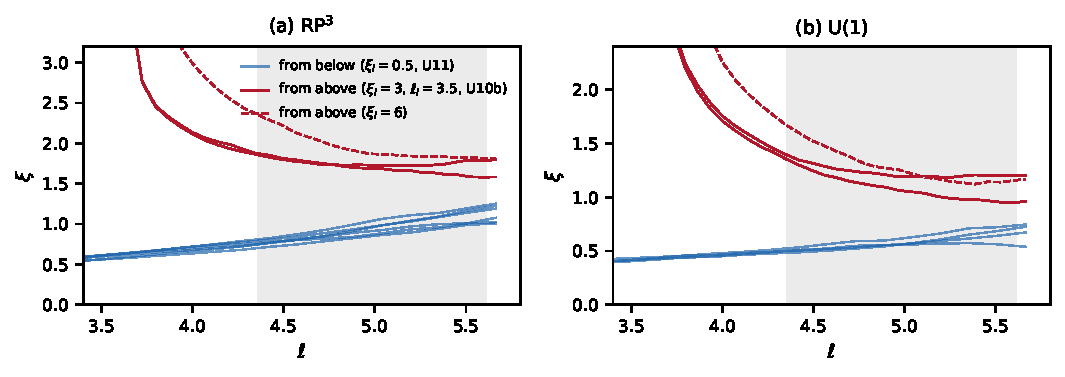
\includegraphics[width=\textwidth]{figures/fig_bracket.pdf}
\caption{The scaling attractor bracketed at $576^3$. Blue: drained networks starting sparse ($\xi_i=0.5$), approaching from below. Red: drained networks started late ($\ell_i=3.5$) and dense ($\xi_i=3$ solid, $6$ dashed), approaching from above. The shaded band is the analysis window. From version~1.}
\label{fig:bracket}
\end{figure}

%=====================================================================
\section{The collapse of the string--wall network}
\label{sec:collapse}
%=====================================================================

\subsection{Why the collapse dominates}

When the walls appear, at $H=m_G/3$, the network energy density is $\rho_{\rm net}=4\xi\pi f_a^2\ell H^2$ and the misalignment energy is $\rho_{\rm mis}=\tfrac38m_G^2F^2$.
At the cosmological $\ell\simeq90$, $\rho_{\rm net}/\rho_{\rm mis}\simeq100$ for a network with constant density and up to $\sim2000$ if $\xi$ grows logarithmically.
If a fraction $\eta$ of that energy ends as Goldstones of mean energy $c\,m_G$, the collapse adds $K=(8\pi/27)\,\xi\ell\,\eta/c$ quanta per misalignment quantum.
Version~1 bracketed this contribution as $K\in\{0,1\}$; the inventory gives $K\sim3$--$800$ depending on $c/\eta$ and on the density branch, and the abundance condition
\begin{equation}
\big[\Omega_{\rm mis}(m_G)\,(1+K) + \Omega_{\rm em}(m_G)\big]\,h^2 = 0.12
\end{equation}
then lowers $m_G$ by two to four orders of magnitude with respect to version~1.
A classic U(1) simulation of the full string--wall system~\cite{Hiramatsu2012} finds a collapse contribution about ten times the misalignment, with mean energy $\simeq3.3\,m_a$ per axion and with all the network energy assumed to end in axions ($\eta=1$), i.e.\ $c/\eta\simeq3$, the warm end of our preregistered range.

Two consequences follow before any Lyman-$\alpha$ computation.
Branches in which the string density keeps growing up to $\ell\simeq90$ need the collapse to put almost all its energy into very hard quanta ($\eta\lesssim0.05$--$0.1$), which no simulation shows: they are disfavoured.
For a constant density (the branch supported by the largest U(1) simulations~\cite{Correia2025spectrum,Correia2024terasite}), what matters for Lyman-$\alpha$ is a single combination: with the population written as a soft part, the suppression depends only on $X=K\,\bar c\,r$, the soft momentum released per misalignment quantum, where $\bar c=\sqrt{c^2-1}$ is the mean momentum in units of $m_G$ and $r$ measures how late the collapse ends.
With the constant-density normalisation at $\ell\simeq90$ and $R_\rho=1.56$,
\begin{equation}
X = \frac{8\pi}{27}\,R_\rho\,\xi_*\ell\;Y \simeq 162\,Y ,
\end{equation}
where $Y$ is the soft yield per unit string energy; a U(1)-like collapse ($\eta=1$, $c=3$, $r=1$) has $Y=0.94$.

\subsection{The collapse measured on the lattice}

To measure $Y$ we evolve the $\RP$ field with the explicit breaking on $512^3$ lattices until the network has disappeared, with two protocols (sparse and dense string densities at the onset of the collapse, $\xi_1\approx0.7$ and $2.4$) and two seeds each, and count the Goldstone quanta of the final state; the counter reproduces the homogeneous equation to $\le1.6\%$, and each network must pass four validity checks (strings and walls gone, no site far from the vacuum, a flat count).
The soft momentum released, in units of $m_G a_1$ per misalignment quantum and with the misalignment population subtracted, is $X_{\rm lat}=\sum_{k<10m_Ga_1}k\,n_k/(m_Ga_1N_{\rm mis})$.
At $\ell_1\simeq4.3$ the preregistered verdict was a soft collapse, $Y=1.70\pm0.55$, but by the narrowest margin (the threshold was $Y-\sigma>1.14$ and the result $1.150$), and two reasonable analysis choices would move it to the intermediate class; we therefore do not lean on the label.
Three findings matter more than the label.
\begin{itemize}
\item \textbf{$\RP$ collapses like U(1).} At $512^3$, the same protocols with a U(1) field in the same code give $Y=1.58\pm0.50$; per protocol and seed the ratio is $1.06$--$1.08$. The $\RP$ network leaves more soft quanta only because it has more strings, and per quantum it is slightly softer (mean momentum $c_p\simeq4.3$ against $5.8$, in units of $m_G$ at the end of the collapse). Our U(1) does not reproduce the analytic U(1)-like collapse ($Y=0.94$); the lattice value is $1.7$ times larger, which may be a property of our small $\ell$ and short mass hierarchy.
\item \textbf{The soft momentum depends little on the string density.} Across protocols, $X_{\rm lat}$ changes by $15\%$ when the string density at the onset changes by a factor $5.5$; the extra energy of dense networks goes into hard quanta, which do not matter for Lyman-$\alpha$. We therefore decompose $X=X_0+y_s\,Z$, with $X_0$ the part independent of the string energy $Z$. A natural reading, not tested, is that the soft quanta come from the walls stretched across the horizon, whose area per Hubble volume is fixed at the horizon scale, while the extra string length of dense networks sits in sub-horizon loops that release hard quanta when the walls pull them in.
\item \textbf{It grows with $\ell$.} $X_0$ is larger at larger $\ell_1$, so the favourable reading in which the soft yield stays at its lattice value ($X\approx8$, cold even at $F_0$) is not supported. How fast it grows decides the band of $F$. Several things change together with $\ell_1$ between our lattices (the hierarchy between the horizon and the core, the epoch at which the collapse ends, the box size in Hubble units), and with these data the growth cannot be attributed to one of them.
\end{itemize}
The collapse ends late: the walls fall to $10\%$ at $a\simeq1.8\,a_1$ and the number of quanta settles at $a\simeq2.4\,a_1$.
The measured spectrum of the soft excess has a mean momentum $\bar x=5.83\,m_Ga_{\rm osc}$, hotter than the log-normal with $\bar x=3$ assumed before it was measured.

\subsection{Extrapolation to $\ell\simeq90$}

Two lattice sizes could not separate extrapolations that grow with $\ell$, and an independent re-analysis showed that our first reading overstated the evidence against a constant $X_0$.
We therefore repeated the protocol at fixed $\ell_G$ relative to $\ell_1$ on four lattice sizes, $256^3$, $384^3$, $512^3$ and $576^3$ ($\ell_1=3.61$, $4.01$, $4.30$, $4.42$; larger lattices fail the counter validation, by $5.4\%$ and $6.5\%$ against $5\%$).
With four networks per mass the masses scattered more than their errors and the exponent was undetermined; the preregistered remedy, twelve networks per mass with the same analysis, gave a smooth, monotonic $X_0(\ell_1)$ (Fig.~\ref{fig:collapse}a):
\begin{equation}
X_0 = 6.49\pm0.32,\ 7.50\pm0.43,\ 8.20\pm0.35,\ 8.57\pm0.42;\qquad X_0\propto\ell_1^{\,p},\ \ p=1.35\pm0.31 .
\end{equation}
The $576^3$ networks were run on a GPU with a JAX port of the kernel that reproduces the C code to machine precision on a control network.
The preregistered extrapolation, $\Xu=X_0(90)+162\max(y_s+2\sigma,0)$ with the least favourable string term ($49$), gives
\begin{equation}
\Xu \simeq 556\qquad (244\text{--}1367\ \text{for}\ p\pm\sigma_p),
\end{equation}
which the verdict logic classifies as undecided because the interval crosses the boundaries it was asked about.
The other models that fit the data give $\Xu\simeq218$ ($X_0\propto\ell_1$) and $273$ (linear in $\ell_1$); a constant $X_0$ ($\Xu\simeq56$) is disfavoured by $\Delta\chi^2\approx19$ (Fig.~\ref{fig:collapse}b).
The data cannot distinguish the three growing forms, because the extrapolation multiplies $\ell$ by more than twenty.
\emph{Informative reading.} In the sparse networks of the four lattice sizes the mean momentum per quantum at the end of the collapse is constant, $c_p\simeq3.49$--$3.55$, while the end of the collapse moves as $r_W\propto\ell_1^{0.53}$; this is the behaviour expected if the walls must first overcome a string tension that grows as $\ell$, which delays the collapse to $H\sim\sigma_w/\mu\propto m_G/\ell$ and gives $r\propto\ell^{1/2}$ in radiation domination, and nothing in this argument saturates at larger $\ell$.
If the network energy is frozen when the walls appear and released at the end of the collapse, the soft momentum grows as $\ell\,r\propto\ell^{3/2}$; if the network keeps scaling, and losing energy, while it waits, it grows as $\ell$.
The fitted exponent, $p=1.35\pm0.31$, lies between these two readings, so the physics does not select among the models that fit any more than the data do; the energy budget, $X\lesssim162\,r$, allows the central extrapolation if $r(90)\gtrsim3.4$, as the $\ell^{1/2}$ delay gives.
All of them give $\Xu>194$, the value below which the benchmark $F_0$ would have passed the Lyman-$\alpha$ screening (\S\ref{sec:band}).

\begin{figure}[t]
\centering
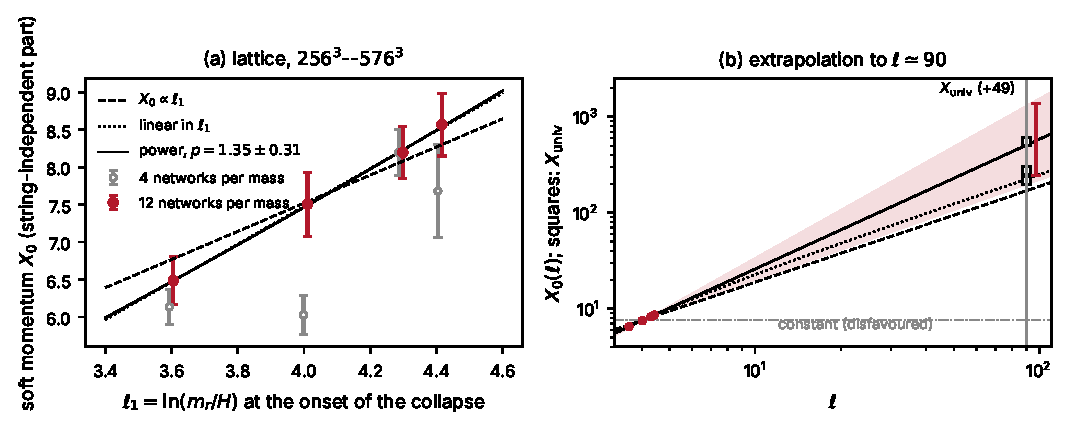
\includegraphics[width=\textwidth]{figures/fig_collapse.pdf}
\caption{The soft yield of the string--wall collapse. (a) String-independent soft momentum $X_0$ against $\ell_1$ at the onset of the collapse, with four (grey) and twelve (red) $\RP$ networks per lattice size, and the three growing models that fit. (b) Extrapolation of $X_0$ to the cosmological $\ell\simeq90$: power law with its $1\sigma$ band, $X_0\propto\ell_1$ (dashed), linear (dotted) and constant (dash-dotted, disfavoured). The squares are $\Xu$ for the three growing models, which include the string term ($+49$); the red bar is the preregistered interval.}
\label{fig:collapse}
\end{figure}

%=====================================================================
\section{Constraints and the band of $F$}
\label{sec:band}
%=====================================================================

\subsection{Gates}

\paragraph{Lyman-$\alpha$ screening.}
The linear transfer function at $z=3$ is computed with CLASS v3.4.1~\cite{CLASSII,CLASSIV}, with the measured distribution read from a file as a non-cold species with the full Boltzmann hierarchy and an 18-line quadrature patch that places nodes uniformly in $\ln q$ (the fixed quadratures and the fluid approximation do not converge for these heavy-tailed distributions; the patched build is validated against analytic Fermi--Dirac and against our own synchronous-gauge solver).
The primary gate is a shape criterion: $T^2(k)$ on $0.5$--$20\,h$/Mpc is fitted with a grid of mixed cold plus thermal-warm models and must satisfy the mixed-dark-matter bound~\cite{GarciaGallego2025} or correspond to a thermal mass $\ge5.3$\,keV~\cite{Irsic2017}.
The area criterion $\dA$~\cite{Murgia2017} is reported with two references computed with the same set-up, strict ($0.234$, a 1\,keV mixed model at the bound) and wide ($0.336$, thermal 5.3\,keV); rows with $\dA$ above the wide reference that pass only the shape gate are marked ``by shape''.
Rows far colder than 5.3\,keV pass without CLASS.

\paragraph{Isocurvature.}
The collapse leaves white-noise isocurvature at scales $k_*\sim a H$ at the collapse, $f_{\rm iso}=C\,(k_{\rm CMB}/k_*)^3/A_s$, with $C=1$ and $k_*$ evaluated at the measured end of the collapse.
The gate is the Lyman-$\alpha$ bound $f_{\rm iso}<0.0084$~\cite{GarciaGallego2026}.
An earlier, self-made criterion was about 500 times stricter than the data and is superseded (appendix).

\paragraph{Black-hole superradiance.}
The primary gate is the $2\sigma$ excluded region from stellar black holes with self-interactions included~\cite{WitteMummery2025,BGLS2021}, with the effective decay constant between $F/4$ and $F$.
The bound from supermassive black holes~\cite{Unal2021,ChathirathasSchwetz2025}, which excludes $m_G<1.7\times10^{-17}$\,eV for our decay constants, rests on a single analysis that others consider less robust; we report it as a secondary bound.

\paragraph{Others.} $\Delta N_{\rm eff}\le0.3$ and the CMB bound on global strings; neither cuts in the band.

\subsection{The band}

With the measured population, the abundance solved for $m_G$ at each $F$, and the five gates, we computed families of rows at fixed $Y$ covering $\Xu$ from 160 to 1370 in two preregistered tests (84 rows through CLASS, the colder ones by the trivial-cold rule). Table~\ref{tab:band} and Fig.~\ref{fig:band} give the band.
In every family the upper edge is set by Lyman-$\alpha$; isocurvature fails only where Lyman-$\alpha$ already fails; the lower edge is set by stellar superradiance, and moves down as $\Xu$ grows because $m_G$ falls.
The dark matter is cold in the whole band and $96$--$99\%$ of it comes from the collapse.

\begin{table}[t]
\centering\small
\caption{Edges of the band of $F$ with the Lyman-$\alpha$ screening gates, against the soft momentum of the collapse in the universe. $^\dagger$: the edge row passes only by shape, with $\dA$ above the wide reference ($0.336$). The last column adds the secondary bound from supermassive black holes. The rows at $\Xu\simeq193$ and $\Xu\simeq320$ were tested with the full likelihood (\S\ref{sec:lyafull}).}
\label{tab:band}
\setlength{\tabcolsep}{4pt}
\begin{tabular}{rcccccc}
\toprule
$\Xu$ & upper edge & $\dA$ there & $m_G$ there (eV) & lower edge & $m_G$ there (eV) & with SMBH\\
\midrule
$\simeq160$--$193$ & $F_0$ & $0.335$--$0.378$$^\dagger$ & $6$--$8\times10^{-18}$ & $0.09F_0$ & $2\times10^{-13}$ & $0.7$--$0.85F_0$\\
$\simeq217$ & $0.85F_0$ & $0.328$ & $8.9\times10^{-18}$ & $0.09F_0$ & $1.3\times10^{-13}$ & $0.7F_0$\\
$\simeq272$ & $0.85F_0$ & $0.383$$^\dagger$ & $5.6\times10^{-18}$ & $0.09F_0$ & $8.4\times10^{-14}$ & $0.5F_0$\\
$\simeq315$ & $0.7F_0$ & $0.323$ & $9.4\times10^{-18}$ & $0.0625F_0$ & $2.8\times10^{-13}$ & $0.5F_0$\\
$\simeq396$ & $0.6F_0$ & $0.301$ & $1.1\times10^{-17}$ & $0.0625F_0$ & $1.8\times10^{-13}$ & $0.5F_0$\\
$\simeq477$ & $0.6F_0$ & $0.350$$^\dagger$ & $7.5\times10^{-18}$ & $0.0625F_0$ & $1.2\times10^{-13}$ & $0.5F_0$\\
$\simeq541$ & $\mathbf{0.5F_0}$ & $0.288$ & $1.3\times10^{-17}$ & $0.0625F_0$ & $9.2\times10^{-14}$ & $0.35F_0$\\
$\simeq674$ & $0.5F_0$ & $0.346$$^\dagger$ & $7.8\times10^{-18}$ & $0.045F_0$ & $2.3\times10^{-13}$ & $0.35F_0$\\
$\simeq859$ & $0.35F_0$ & $0.231$ & $2.3\times10^{-17}$ & $0.045F_0$ & $1.4\times10^{-13}$ & $0.35F_0$\\
$\simeq1333$ & $0.35F_0$ & $0.336$$^\dagger$ & $8.5\times10^{-18}$ & $0.03F_0$ & $3.1\times10^{-13}$ & $0.25F_0$\\
\bottomrule
\end{tabular}
\end{table}

\begin{figure}[t]
\centering
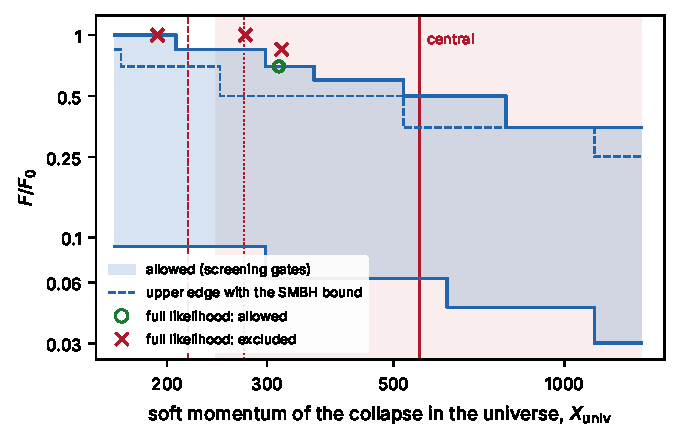
\includegraphics[width=0.72\textwidth]{figures/fig_band.pdf}
\caption{The band of $F$ against $\Xu$. Shaded: allowed by the Lyman-$\alpha$ screening, isocurvature, stellar superradiance, $\Delta N_{\rm eff}$ and CMB string gates; dashed: upper edge with the secondary supermassive black-hole bound. Vertical lines: the central extrapolation of the collapse (solid), $X_0\propto\ell_1$ (dashed) and linear (dotted); the light band is the preregistered interval. Markers: the four rows tested with the full Lyman-$\alpha$ likelihood.}
\label{fig:band}
\end{figure}

\subsection{The full Lyman-$\alpha$ likelihood}
\label{sec:lyafull}

The screening gates compare a transfer function with a family of thermal models at fixed cosmology.
We also ran the full likelihood of Ref.~\cite{Hooper2022}, with Planck 2018 (high-$\ell$ lite and low-$\ell$)~\cite{Planck2018V}, BAO~\cite{Alam2017} and the Lyman-$\alpha$ flux power spectrum, sampling the cosmological and intergalactic-medium parameters with MontePython~\cite{MontePython2019}.
Each case enters with a free amplitude $s$ of its non-cold component, $\omega_{\rm ncdm}=s\,f_{\rm nc}\,\Omega_{\rm DM}$ (so $s=0$ is cold dark matter and $s=1$ the model), with a flat prior on $[0,1/f_{\rm nc}]$ and $T^2(k;s)$ tabulated with CLASS.
A case is allowed if $p(s=1)/p_{\max}\ge e^{-2}$ with 30 bins, and undecided if the label changes with 20 or 45 bins or when one of the four chains is removed; the chains must reach $R-1<0.03$ in every parameter, also in halves.
The harness was validated with thermal mixtures, whose $95\%$ limits on the warm fraction, $0.27$ (1\,keV) and $0.42$ (2\,keV), fall inside the preregistered windows around the published fit.

The first two cases tested the band edges of an earlier stage with the log-normal population ($0.5F_0$ and $0.35F_0$): both pass with $p(s=1)/p_{\max}=0.87$ and $0.91$, but only because their suppression at $k=10\,h$/Mpc is below $0.15\%$, 50--100 times below what the data detect, so the posterior of $s$ is flat.
The decisive cases use the measured population at the upper edge (Fig.~\ref{fig:lyafull}):

\begin{table}[h]
\centering\small
\begin{tabular}{lcccccc}
\toprule
Case & $\Xu$ & $T^2(k{=}10\,h/{\rm Mpc})$ & $p(s{=}1)/p_{\max}$ & 20 / 45 bins & one chain removed & label\\
\midrule
$F_0$ & 193 & 0.972 & $0.111$ & $0.116$ / $0.126$ & $0.106$--$0.117$ & excluded\\
$F_0$ & 275 & 0.946 & $0.047$ & $0.045$ / $0.044$ & $0.038$--$0.057$ & excluded\\
$0.85F_0$ & 318 & 0.961 & $0.114$ & $0.112$ / $0.113$ & $0.110$--$0.120$ & excluded\\
$0.7F_0$ & 315 & 0.982 & $0.238$ & $0.239$ / $0.242$ & $0.225$--$0.246$ & allowed\\
\bottomrule
\end{tabular}
\end{table}

All four converged with four chains ($R-1\le0.017$, $\le0.026$ in halves; $\simeq1.8$--$2.0\times10^5$ points each) and no label changes with the binning or the jackknife.
The preregistered verdict is that the benchmark is excluded by the full likelihood and the $0.7F_0$ edge holds at $\Xu\simeq320$; the specification expected the benchmark to pass at $\Xu\simeq195$, on the basis of the calibration of the thermal validation, and that expectation failed.
The two exclusions at $0.11$ are close to the threshold ($-2\ln p=4.3$--$4.4$ against $4$), comparable to the bound on the error of evaluating $T^2$ at a fiducial cosmology ($|\Delta\ln L|\approx0.4$--$0.7$).
The posterior of $s$ is no longer flat: it decreases monotonically from $s\approx0$, so the data prefer cold dark matter to these rows, more strongly the larger the suppression.

\emph{Informative reading.} The row that passes has screening $\dA=0.323$ and the excluded ones $0.378$ and above, so the full likelihood cuts between $\dA\approx0.32$ and $0.38$; $\dA$ does not order the cases strictly (the rows with $0.378$ and $0.421$ give the same $p(s=1)/p_{\max}$), because the likelihood sees the full shape and redshift dependence.
The screening gate is therefore not conservative for rows that pass by shape only: the five rows marked so in Table~\ref{tab:band} become doubtful, and their edge may move down one step of the grid.
The central row ($\Xu\simeq541$, $0.5F_0$, $\dA=0.288$) is not affected.

\begin{figure}[t]
\centering
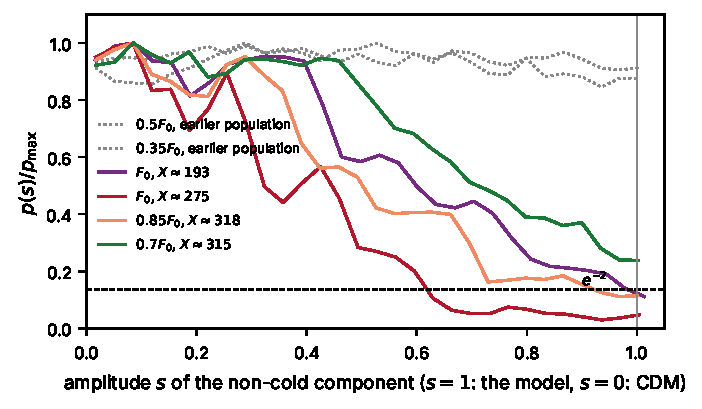
\includegraphics[width=0.72\textwidth]{figures/fig_lyafull.pdf}
\caption{Posterior of the amplitude $s$ of the non-cold component with the full Lyman-$\alpha$ likelihood (Planck + BAO + Lyman-$\alpha$, cosmology and intergalactic medium marginalised), normalised to its maximum. Dotted: two band edges with the earlier log-normal population, indistinguishable from cold dark matter. Solid: the measured population at the upper edge. The dashed line is the preregistered threshold $e^{-2}$ at $s=1$.}
\label{fig:lyafull}
\end{figure}

\subsection{Best estimate}

Combining the band with the extrapolation of the collapse:
\begin{itemize}
\item at the central extrapolation ($\Xu\simeq556$), $F\approx0.06$--$0.5F_0$, i.e.\ $f_a\approx0.3$--$2.7\times10^{14}$\,GeV and $m_G\approx1.3\times10^{-17}$--$9\times10^{-14}$\,eV, with the oscillation starting at $T\approx0.1$--$8$\,MeV; with the supermassive black-hole bound, $0.06$--$0.35F_0$;
\item over the whole preregistered interval of the collapse, $F\approx0.03$--$0.85F_0$, where $0.85F_0$ survives only near $\Xu\simeq220$ and with $\dA$ at the edge of what the full likelihood allows;
\item $F_0$, and with it the benchmark of version~1, is excluded unless the soft yield grows more slowly than every model that fits: the full likelihood excludes it already at $\Xu\simeq193$, and the fitted models give $\Xu\ge218$. The two arguments are complementary, not independent: both assume a growing yield.
\end{itemize}

%=====================================================================
\section{Predictions and falsifiers}
\label{sec:predictions}
%=====================================================================

\begin{table}[t]
\centering\small
\caption{Predictions of the model and what would falsify them. The dark-sector entries assume the central extrapolation of the collapse unless stated.}
\label{tab:predictions}
\begin{tabular}{L{3.0cm}L{5.4cm}L{5.6cm}}
\toprule
Observable & Prediction & Falsified or put under strain by\\
\midrule
Scalar tilt & $n_s = 0.9728$ & $n_s$ outside $\sim0.965$--$0.98$ at $\sigma\lesssim0.002$\\
Tensor ratio & $r = 0.0050$ & $r<0.003$ (LiteBIRD, CMB-S4); $r\lesssim10^{-3}$ falsifies the whole model\\
Large-scale anomalies & none from the bounce: in the eternal branch, and in every direct child of the archived grid ($\gtrsim108$ e-folds), the bounce lies far outside the observable universe & an imprint would need a direct child landing below $\approx4.1\,\Mpl$, which the grid does not sample and whose imprint is not computed\\
Dark-matter nature & cold pseudo-Goldstones, $96$--$99\%$ from the string--wall collapse & a warm or hot dark-matter component detected in the small-scale power\\
Goldstone mass & $m_G\approx10^{-17}$--$10^{-13}$\,eV ($1.3\times10^{-17}$--$9\times10^{-14}$\,eV central) with $f_a\approx0.3$--$2.7\times10^{14}$\,GeV & superradiance or other ultralight-boson bounds closing this window at these decay constants\\
Small-scale power & suppression at most a few per cent at $k=10\,h$/Mpc near the upper edge ($T^2\approx0.98$ at the edge allowed by the full likelihood), vanishing towards the lower edge & a detected suppression larger than the upper edge allows is not produced by this sector; no detected suppression is consistent with lower $F$\\
Isocurvature & white noise at $k\gtrsim10^3$\,Mpc$^{-1}$, $f_{\rm iso}\approx5\times10^{-4}$ at the upper edge for the central $\Xu$ and up to $1.6\times10^{-3}$ over the interval ($C=1$), negligible towards the lower edge & a confirmed $f_{\rm iso}\approx0.006$ (the tentative Lyman-$\alpha$ detection~\cite{GarciaGallego2026}) fits only near $F_0$, which is excluded, unless $C\gg1$\\
Dark radiation & $\Delta N_{\rm eff}\lesssim3\times10^{-3}$ & a detected $\Delta N_{\rm eff}\gtrsim0.05$ is not produced by this sector\\
Gravitational waves & global strings with $f_a\lesssim2.7\times10^{14}$\,GeV: below the LISA threshold~\cite{GHN2021} & a LISA global-string background (it would need $f_a\gtrsim5\times10^{14}$\,GeV)\\
Collapse at large $\ell$ & soft yield growing as $\ell^{1.35\pm0.31}$, $\Xu\simeq244$--$1370$ & a yield growing more slowly than $\ell_1$ (a constant one is disfavoured by $\Delta\chi^2\approx19$) would bring $F_0$ back below $\Xu\approx190$, where the full likelihood was not tested\\
Miniclusters & characteristic masses $\sim10^{-3}$--$10^{4}\,M_\odot$ across the band ($5\times10^3$ to $8\times10^{-3}\,M_\odot$ at the central $\Xu$), from the literature scaling $M\propto m_G^{-3/2}$; uncertain by about an order of magnitude & not computed as a population; the microlensing bound of version~1 is not recomputed\\
\bottomrule
\end{tabular}
\end{table}

Table~\ref{tab:predictions} lists the predictions.
The inflationary ones have no free parameter once $V_0$ is fixed.
The dark-sector ones are a band rather than a point because $F$ is free below its ceiling and the collapse is extrapolated over a factor of twenty in $\ell$.
Unlike version~1, survival no longer hinges on one side of the dispute about the large-$\ell$ behaviour of global-string radiation~\cite{GHV2021,Buschmann2022,KimParkSon2024,Saikawa2024,Benabou2025,Correia2025spectrum}: with the collapse dominating, the slope of that radiation is irrelevant, and a constant string density is still assumed because the growing branches need an implausibly hard collapse.
The band does not close at any $\Xu$ we tested: what would remove the dark sector is a combination of tighter superradiance bounds at the lower edge and tighter small-scale or isocurvature bounds at the upper edge.

%=====================================================================
\section{Open assumptions}
\label{sec:open}
%=====================================================================

\begin{description}
\item[Seed.] The small, closed, contracting patch is assumed, not derived; it needs to exist only once. The interior of a regular black hole in NPQT gravity, a closed contracting region causally separated from its exterior, is a candidate origin that has not been computed; it would have to avoid the incoherence that spoils local collapses in an expanding parent (\S\ref{sec:birth}), for example by being causally separated by the horizon.
\item[Field range.] Eternal inflation in the landing zone needs a plateau flat to $1.2\times10^{-6}$ per $\Mpl$ up to $\chi\sim10^3\Mpl$. We know of no UV construction that protects this; axion monodromy controls ranges of $\sim10\Mpl$, and the distance and de Sitter swampland conjectures~\cite{Obied2018} exclude it. The model lives outside the swampland or not at all. The shape of the plateau, a postulated hierarchy in version~1, is now a standard pole, which makes the required flatness stable against corrections analytic at the pole (\S\ref{sec:pocket}); what remains assumed is that the ultraviolet completion respects the pole over a geodesic range of $\sim10^3\Mpl$. The requirement belongs to the eternal branch: if our pocket is a direct, non-eternal child, the branch that the coherence of the parent's bounces favours (\S\ref{sec:birth}), the plateau needs to be flat only up to its landing value, $10$--$50\,\Mpl$ for at least $4.0\%$ of fertile births, still a super-Planckian range for the distance conjecture. A bounce within reach of the largest observable scales would need a landing below $\approx4.1\,\Mpl$, with at most $\approx60$ e-folds in total; the archived grid does not sample such births (its fertility criterion requires the field to exceed $5\,\Mpl$ after the bounce, which already gives $\approx108$ e-folds), and the imprint has not been computed.
\item[Measure.] The fraction of births that land in the eternal regime depends on the prior over parent states, not on a measure; weights within eternal inflation are measure-dependent, and so is whether observers live in pockets of the eternal branch or in direct children. Once eternal inflation is reached, volume favours the eternal branch; the coherence of the parent's bounces favours direct children ($12.4$--$18.0\%$ of fertile births against $1.8$--$2.9\%$, \S\ref{sec:birth}). The predictions are not: every pocket and every direct child with more than $\sim60$ e-folds exits along the same single-field attractor, with the same $n_s$, $r$ and dark sector at a given $F$.
\item[Quantum backreaction at birth.] The contraction, bounce and kick are computed with a classical homogeneous $\chi$. Whether the quantum state of its zero mode, with its backreaction on $Q$, radiation and the NPQT background, follows the same history through the bounce and the launch is not established; a single mean background with fluctuating stress is itself an approximation near the bounce.
\item[Perturbations in NPQT.] Linear perturbations are not computed; standard perturbation theory on the NPQT background is assumed during inflation. At the bounce of the parent, where $\alpha\psi\to1$, the coherence test evolves spherical inhomogeneities nonlinearly with the NPQT equations (\S\ref{sec:birth}); non-spherical modes are not computed. During eternal and observable inflation $\alpha\psi=\alpha V_0/3\lesssim4\times10^{-4}$ for the viable children, so the background is that of general relativity to $\alpha^2\psi^2\lesssim2\times10^{-7}$; the CMB predictions rest on the theory reducing smoothly to general relativity at low curvature.
\item[Multi-bounce coherence.] Computed with an inhomogeneous $\chi$ for one bounce, in spherical symmetry and at one perturbation scale ($L\cdot H=1$), and extrapolated to several bounces by dividing the tolerated amplitude by their number, as in the dust model: the direct branch is viable and the eternal one marginal (\S\ref{sec:birth}). At the shorter scale $L\cdot H=0.3$ more than $20\%$ of the runs fail numerically, and the test is inconclusive there; in the dust model that scale leaves $2.2\%$ direct and $1.1\%$ eternal children.
\item[Closing the loop.] Inflating islands seen from neighbouring pockets as black holes containing new eternal regions~\cite{GVZ2016}: an argument, without calculation. It is not needed for the model to exist: once reached, eternal inflation perpetuates itself.
\item[$m_G$.] A bare, technically natural parameter of the effective theory; no ultraviolet origin is built, and Planck-suppressed breaking must be forbidden, for instance by a discrete gauge symmetry (\S\ref{sec:F}).
\item[$F$ and the ordering of $Q$.] $F$ is free below $F_0$; the delayed ordering at small $F$ (at most $\simeq2$ e-folds) is argued, not computed, to leave the network at $\ell\approx80$--$90$ unchanged (\S\ref{sec:F}).
\item[The collapse at $\ell\approx90$.] The soft yield is measured at $\ell_1\le4.42$ and extrapolated to $\ell\simeq90$; three growing forms fit equally well and give $\Xu$ from 218 to 556, with a preregistered interval up to 1370. The energy ratio $R_\rho$ of $\RP$ to U(1) strings is taken equal to the emission ratio; it enters only the string term of $\Xu$ ($49$ of the central $556$), because $X_0$ is measured on the $\RP$ lattice itself. Our lattice U(1) collapse is softer than the analytic U(1)-like one by a factor $1.7$ in $Y$; if the lattice overestimates $Y$ in both models, the band would move up.
\item[Isocurvature normalisation.] $C=1$ is not computed; with $C\gg1$ isocurvature would cut the upper edge. Our collapse lattices cannot measure it: at the end of the collapse they span only about one and a half Hubble volumes, so the white-noise plateau at $k\ll aH$ is outside the box, and the stored results keep the Goldstone number spectrum, not the density field. Measuring $C$ needs boxes many Hubble volumes across at the end of the collapse.
\item[Superradiance.] The stellar region is a digitised figure ($\pm0.1$\,dex); the supermassive bound rests on one analysis.
\item[Full likelihood beyond $\Xu\simeq320$.] The rows that pass the screening by shape only, at $\Xu\simeq272$ and $477$--$1333$, have not been tested with the full likelihood; $T^2$ is evaluated at a fiducial cosmology, and with $f_{\rm nc}\simeq0.98$ the model lies near the edge of the simulations behind the likelihood, although none of its internal range checks was triggered in any chain.
\item[Reheating bath.] Reheating uses an effective friction; the bath model and preheating are not computed.
\end{description}

%=====================================================================
\section{What changed since version 2}
\label{sec:changes3}
%=====================================================================

Version~2 (25 October 2026) is kept unchanged as the record of the dark sector, which this version does not modify: the CMB predictions, the collapse, the band of $F$ and the full likelihood are the same.
The following statements of version~2 no longer hold:
\begin{itemize}
\item \emph{We place our pocket in the eternal branch, which dominates by volume.} Both branches remain; volume favours the eternal one, and the coherence of the parent's bounces favours direct children (\S\ref{sec:open}).
\item \emph{$3.6\%$ of fertile children bounce coherently (marginal); the coherence model is dust-only, and coherence with an inhomogeneous $\chi$ is set up but not run.} With the pole plateau, the dust model gives $3.6\%$ eternal and $14.9\%$ direct children; with an inhomogeneous $\chi$, $1.8$--$2.9\%$ eternal (marginal) and $12.4$--$18.0\%$ direct (viable) (\S\ref{sec:birth}).
\item \emph{Perturbations in NPQT are not computed.} The bounce of the parent with spherical inhomogeneities is computed nonlinearly; linear perturbations during inflation still are not.
\item \emph{The plateau must be flat up to $\sim10^3\Mpl$.} Only in the eternal branch; a direct child needs it flat up to its landing value, $10$--$50\,\Mpl$ for at least $4.0\%$ of fertile births.
\end{itemize}

%=====================================================================
\section{What changed since version 1}
\label{sec:changes}
%=====================================================================

Version~1 is kept unchanged as the historical record.
The following statements of version~1 no longer hold:
\begin{itemize}
\item \emph{The string--wall collapse brackets as $K_{\rm sw}\in\{0,1\}$.} It carries $10^2$--$10^3$ times the misalignment energy and sets the abundance (\S\ref{sec:collapse}).
\item \emph{$m_G\approx0.8$--$5\times10^{-15}$\,eV, $15$--$59\%$ emitted by the network, $\dA\approx0.08$--$0.22$.} With the collapse, the emission before it is below $0.02\%$ of the dark matter, and $m_G\approx10^{-17}$--$10^{-13}$\,eV depending on $F$.
\item \emph{Survival hinges on the slope $q$ at large $\ell$ (critical values $1.025$ and $0.91$), with a warm branch for $q\simeq1$ and a cold one for $q<1$.} The slope no longer decides anything; the dark matter is cold in the whole band.
\item \emph{$F\simeq1.07\times10^{15}$\,GeV, fixed.} $F$ is a free parameter with that value as its ceiling, and the ceiling itself is excluded.
\item \emph{Global strings near the LISA threshold.} With $F$ in the band the string background is below it.
\item \emph{The mass sits in the gap between the superradiance windows.} Stellar superradiance sets the lower edge of the band, and the supermassive bound a secondary upper one.
\item \emph{Isocurvature at most $2.5\times10^{-3}$ of the adiabatic power.} That was the network emission alone; the collapse gives $f_{\rm iso}$ of $5\times10^{-4}$--$1.6\times10^{-3}$ at the upper edge, below the Lyman-$\alpha$ bound and near the contested bound from ultra-faint dwarfs ($6\times10^{-4}$).
\item \emph{The ten-level plateau is postulated.} It is replaced by a standard pole with the same observables.
\item \emph{Miniclusters of $\sim0.2$--$10\,M_\odot$ and their microlensing bound.} They were computed for the version-1 masses; with the literature scaling the band gives $\sim10^{-3}$--$10^4\,M_\odot$, and the microlensing bound has not been recomputed.
\item \emph{$\RG=1.56\pm0.09$ as the total error; $q<1$.} The error is $\pm0.12$ with snapshot sampling, and $q$ is compatible with 1 (\S\ref{sec:network}).
\item \emph{An audit of the later stages in progress.} Done, with the corrections it found reported.
\end{itemize}

%=====================================================================
\section{History: what was discarded}
\label{sec:history}
%=====================================================================

Four earlier models (September 2026) explored variants of the $\RP$ scar network, pseudo-Goldstone dark matter and the hierarchical plateau, many discarded by preregistered tests.
The present model (2--4 October 2026) replaced the birth mechanism after the following no-gos:
children born from local collapses inside an expanding parent never bounce coherently;
rescues with sharp, tension-bounded edges fail because tension makes the wall fall faster than dust;
a core--envelope pair cannot play the role of the two centres that generate the $1/\chi$ plateau;
inflated universes cannot be parents of new seeds;
and scars or bubbles fall short by more than $4\times10^3$ in energy as a seed factory.

The dark sector was then tested in stages.
The first closure found a narrow conditional window if the network emitted at most $0.1$--$6\%$ of a U(1) network; the first lattice measurement gave an emission ratio far above that, so the closure with the measured efficiency failed in its original form, and the warmth gate was replaced by a Boltzmann transfer and Lyman-$\alpha$ gates.
Version~1 reported the state after the lattice emission was measured and the initial bath identified (11 October).
On 12 October the energy inventory at the collapse showed the bracket $K_{\rm sw}\in\{0,1\}$ to be untenable; the following week turned the collapse into a population, passed it through CLASS, found that $F$ is a ceiling rather than a fixed value, and added isocurvature and superradiance, first with self-made criteria that later proved too strict or too weak and were replaced by observational bounds.
From 16 October the collapse was measured on the lattice, first at one mass, then two, four, and four with twelve networks each, while the band was recomputed with each new extrapolation and its edge finally tested with the full likelihood.
Appendix~\ref{app:log} lists every test.

%=====================================================================
\section{Reproducibility}
%=====================================================================

The repository~\cite{whalefall_chain}, a one-way export of the working repository with the source commit and the SHA-256 of every file, contains the chain, the coherence codes of the birth (with the original code of the dust model and every run with an inhomogeneous $\chi$), the lattice code with every collapse network and the summary of each emission test (the emission networks one by one are in the repository of the companion paper~\cite{rp3_paper}, \url{https://github.com/indigenica/whalefall-rp3-string-networks}), the CLASS patch and Lyman-$\alpha$ pipelines, the full-likelihood harness, the common-action symbolic checks, frozen inputs from earlier campaigns with SHA-256 provenance, every preregistration with its amendments and the report of each test, and the scripts that produce the figures of this paper from result files only.
\begin{itemize}
\item The coherence tests of the birth run on one core of the cloud machine: that of direct children in $\sim4$\,min, and the $780$ runs of the parent with an inhomogeneous $\chi$ in $\sim3$\,h.
\item \texttt{make test} ($\sim3$\,min) and \texttt{make chain} ($\sim4$\,min) reproduce the chain and the contract on a laptop; the chain runs with the pole plateau by default and with the ten-level hierarchy on request.
\item Lattice runs used a 44-thread workstation, a 4-core cloud machine and, for the largest collapse networks, an A100 GPU with a JAX port of the kernel; the collapse networks took 0.4--2.6\,h each on the cloud machine and the GPU and 9--11\,h each at $512^3$ on the workstation, and each $\RP$ emission network at $576^3$ 1.5--2\,h.
\item CLASS v3.4.1 (commit \texttt{814ce59}) with the patch, which the environment check and the latest CLASS scripts verify before running. The full-likelihood chains (MontePython with Planck lite, BAO and Lyman-$\alpha$) took several days per campaign on the workstation; they are kept by the author and their summaries are in the repository.
\end{itemize}

%=====================================================================
\section*{Acknowledgments}
%=====================================================================

The author thanks the developers of CLASS and MontePython for making their codes public.

Most of the code, the preregistration documents, the audits and the revisions of this text were produced in an iterative workflow with an AI assistant (Claude, Anthropic), under the direction of the author, who chose the scientific questions, the model ingredients, the order of tests and which results to accept.
The audits were carried out by separate sessions of the same assistant, without the audited code, and the external reviews included assistants of other providers (Codex, OpenAI; Gemini, Google), in a red-teaming approach.
The author takes full responsibility for the content.

This research received no external funding, and none is currently in place; support to continue it would be welcome.

\appendix
%=====================================================================
\section{Test log}
\label{app:log}
%=====================================================================

Verdict labels are kept in the original (Spanish) form used in the specifications and result files; the internal codes index the repository.
Tests up to U15 are listed in version~1; those that still bear on the model are repeated here.

\begin{small}
\begin{longtable}{L{1.3cm}L{6.0cm}L{7.0cm}}
\toprule
Test & Question & Preregistered verdict (and later reading)\\
\midrule
\endfirsthead
\toprule
Test & Question & Preregistered verdict (and later reading)\\
\midrule
\endhead
\bottomrule
\endfoot
U11 & Emission with the initial bath drained ($576^3$) & \textsc{limpia\_zona\_permitida} ($\RG=1.56\pm0.09$); \textsc{q\_menor\_que\_1} (later: convention dependent, $q$ compatible with 1) \\
U10b & Late dense starts, approach from above & \textsc{atractor\_acotado}, $\Rxi\in[1.57,1.68]$ \\
U13 & $m_G$ from the common action & \textsc{m\_g\_requiere\_ruptura\_nueva} \\
U15 & Lyman-ABGD likelihood at fixed cosmology & \textsc{inconcluso} (harness failed its validation) \\
U16 & Resolution and volume of the network ratios & \textsc{resolucion\_robusta} ($\Rxi$, $\RG$); volume: \textsc{volumen\_robusto} ($\RG$), \textsc{indeterminado} ($\Rxi$, no power) \\
U18 & Resolution with dense snapshots & \textsc{indeterminado}; snapshot-sampling systematic of $\pm5\%$ adopted after the data \\
U24 & Dependence of $\RG$ on the drain & \textsc{drenaje\_robusto} (at most $1.9\pm1.4\%$) \\
U25 & Time step of the production runs & \textsc{paso\_robusto} \\
U17 & Network energy at the collapse & \textsc{k\_sw\_fuera\_del\_rango\_tibia}: $K\sim3$--$770$, not $0$--$1$ \\
U17b & Collapse population through CLASS & \textsc{solo\_xi\_constante\_vive} \\
U17c & Critical collapse fraction for growing density & \textsc{rama\_comoda\_forzada} ($\eta_{\rm crit}\simeq0.1$; 0.05 for $\xi\propto\ell$) \\
U17d & Corrected balance with $R_\rho=1.56$ & \textsc{rama\_viva\_con\_colapso\_tipo\_u1} (passes by shape only; expectation failed) \\
U21 & Band of $F$ & \textsc{banda\_bajo\_el\_benchmark} ($F\le0.7F_0$; the benchmark fails) \\
U20 & Own isocurvature estimate & \textsc{isocurvatura\_recorta\_banda} (later: criterion $\sim500\times$ stricter than the data; superseded by U20b) \\
U22 & Pole plateau & \textsc{polo\_cambia\_nacimiento} (later: a counting error; corrected by U22b) \\
U22b & Birth statistics with the pole, full grid & \textsc{nacimiento\_robusto} ($R=0.94$) \\
U26 & Pole plateau adopted in the chain & \textsc{polo\_adoptado} \\
U19 & First collapse test ($320^3$) & \textsc{indeterminado} (counter not valid at that size) \\
U19b & Collapse of $\RP$ measured ($512^3$, 4 networks; U(1) control and a second mass) & \textsc{colapso\_blando}, by a margin of $0.01$ (later: fragile; $\RP\simeq$ U(1) per string energy; soft momentum depends little on $\xi$ and grows with $\ell$) \\
U17e & Measured population through CLASS & \textsc{banda\_recortada} \\
U23 & Superradiance with self-interactions & \textsc{superradiancia\_parte\_la\_banda} (stellar BHs set the lower edge) \\
U20b & Isocurvature with observational bounds & \textsc{isocurvatura\_no\_limita} \\
U17f & Upper edge over $\Xu\approx170$--$320$ & \textsc{borde\_0.7\_confirmado}; $F_0$ permitted for $\Xu\le194$, by shape (later: excluded by U15d) \\
U15b & Full Lyman-$\alpha$ likelihood: validation & \textsc{detenido} (physical rows stopped when superseded); validation passed ($f_{95}=0.27$, $0.42$) \\
U15c & Full likelihood at the earlier band edges & \textsc{rama\_viva\_permitida\_lya\_completo} (indistinguishable from CDM) \\
U19c & Collapse at four lattice sizes, 4 networks each & \textsc{indeterminado} ($\sigma_p=0.76$) \\
U19d & Same with 12 networks per size & \textsc{x\_univ\_indeciso} ($\Xu=244$--$1367$; $p=1.35\pm0.31$) \\
U17g & Upper edge over $\Xu\approx400$--$1370$ & \textsc{borde\_baja\_a\_0.35} ($0.5F_0$ at the central $\Xu$) \\
U15d & Full likelihood at the upper edge & \textsc{f0\_excluido\_lya\_completo}; \textsc{borde\_0.7\_sostenido} \\
U27 & Coherence of direct (non-eternal) children with the pole plateau, dust model & \textsc{rama\_directa\_viable}; \textsc{banda\_10\_50\_poblada} ($14.9\%$ direct, $3.6\%$ eternal, $4.9\%$ direct at $10$--$50\,\Mpl$) \\
U28 & Coherence of the parent's bounces with an inhomogeneous $\chi$ & \textsc{igual} in both classes; direct branch \textsc{viable} ($12.4$--$18.0\%$), eternal \textsc{marginal} ($1.8$--$2.9\%$); the preregistered solver could not cover the patch and was replaced before production \\
\end{longtable}
\end{small}

\bibliographystyle{unsrtnat}
\bibliography{refs}

\end{document}
